\documentclass[10pt]{article}
\usepackage{ctex}
\usepackage{CJK}
\usepackage{graphicx}
\bibliographystyle{plain}
\setlength{\parindent}{2em}
\begin{document}
\title{Continous bistable system}
\author{Qilei Zhang}
\date{may 23 2018}
\maketitle
\par
\section{INTRODUCTION}
A two-state description of stochastic resonance is of limited use for a number of reasons. First, the dynamics is reduced to the switching mechanism between two metastable states only\cite{higbibtex}. Thus it neglects the short-time dynamics that takes place within the immediate neighborhood of the metastable states themselves.
\par
\begin{figure}[htbp]
\small
\centering
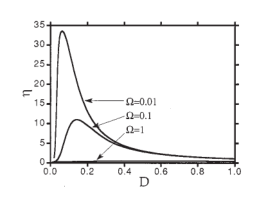
\includegraphics[width=20em]{000.png}
\caption{Continous  bistable  system}
\label{fig:lable}
\end{figure}
\section{CHARACTERIZATION OF STOCHASTIC RESONANCE}
Stochastic resonance was quantified by the intensity of a peak in the power spectrum. Observables based on the power spectrum are indeed very convenient in theory and experiment, since they have immediate intuitive meaning and are readily measurable. First, the important quantifiers based on power spectrum stochastic resonance are discussed. With the introduction of quantifiers\cite{higham1994bibtex}, we prove their properties of the two general models of stochastic resonance, periodically driven bistable two fluid system and Shuangjing system.
\par
Moreover,our goal is to describe both the linear as well as the nonlinear stochastic resonance response in the whole regime of modulation frequencies, extending from exponentially small Kramers rates up to intrawell frequencies, and higher. Put differently, a more elaborate approach has to model the nonadiabatic regime of driving in the whole accessible state space of the dynamical process x(t). This goal will be presented within the class of continuous-state random systems , which can be modeled in terms of a Fokker-Planck equation.
\section{Linear-response theory}
As detailed in the Introduction, the prominent role of the stochastic resonance phenomenon is that it can be used to boost weak signals embedded in a noisy environment\cite{hibibtex}. Thus the linearresponse concept, or more general, the concept of perturbation theory for spectral quantities like the Floquet modes and the Floquet eigenvalues as discussed in the previous section are adequate methods for studying the basic physics that characterizes stochastic resonance.\\
\par
$X(t)=-H(t)\sum_{n=1}^\infty g_n l_n exp(-l_n t)$\\
\bibliography{qaz}
\end{document}

